\begin{frame}{Resultados de la Estimación y Comparación}

    \begin{columns}[T]
        %========================================
        % COLUMNA IZQUIERDA: MÉTRICAS Y GRÁFICA
        %========================================
        \column{0.48\textwidth}
        \begin{block}{Convergencia Numérica}
            \scriptsize
            El algoritmo Nelder-Mead convergió a un residuo óptimo:
            \[ E_{min} \approx 2.8592 \times 10^{-5} \]
        \end{block}

        \vspace{0.1cm}
        
        \begin{center}
            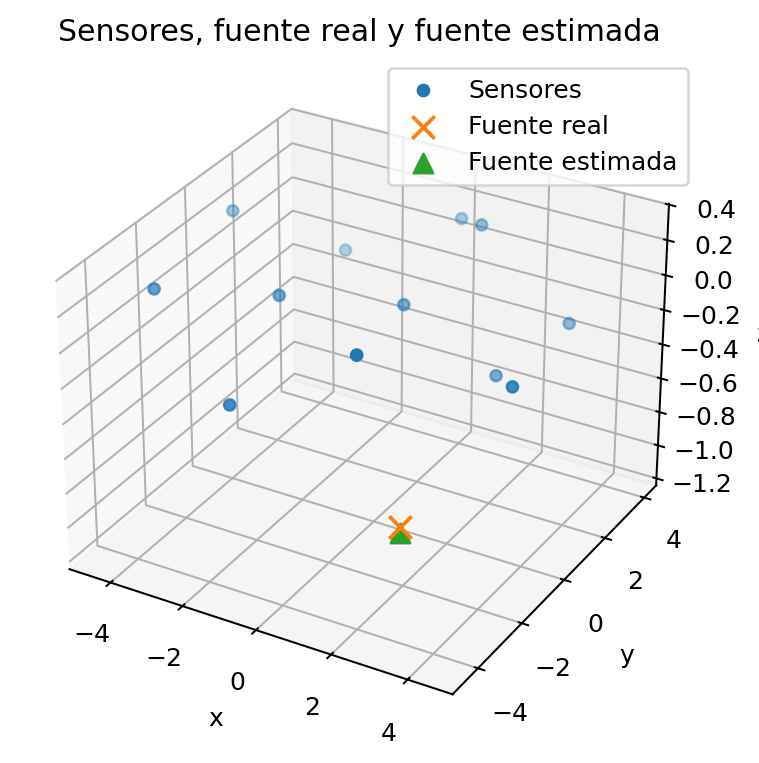
\includegraphics[width=0.9\textwidth]{Imagenes/EstimacionValidacion.png}
            \\ \tiny \textcolor{gray}{Comparativa visual: Fuente Real vs Estimada.}
        \end{center}

        %========================================
        % COLUMNA DERECHA: TABLA COMPARATIVA
        %========================================
        \column{0.48\textwidth}
        \begin{block}{Comparación Definitiva}
            \centering
            \scriptsize
            \begin{tabular}{@{}lccc@{}}
                \toprule
                \textbf{Par.} & \textbf{Real} & \textbf{Est.} & \textbf{Dif.} \\ \midrule
                $x$ & 1.2000 & 1.2001 & 0.0001 \\
                $y$ & -0.8000 & -0.7765 & 0.0235 \\
                $z$ & -1.1000 & -1.1381 & 0.0381 \\ \bottomrule
            \end{tabular}
            
            \vspace{0.2cm}
            \textbf{Distancia neta:} \\
            $\Delta \approx 0.0448$ unidades
        \end{block}

        \begin{block}{Interpretación Física}
            \scriptsize
            Las desviaciones en $y$ y $z$ son consistentes con la perturbación gaussiana del 5\% aplicada al modelo.
        \end{block}
    \end{columns}

\end{frame}